%%%%%%%%%%%%%%%%%%%%%%%%%%%%%%%%%%%%%%%%%%%%%%%%%%%%%%%%%%%%
% NEURIPS 2025 PAPER — Neural Surrogate MILP Solver
%%%%%%%%%%%%%%%%%%%%%%%%%%%%%%%%%%%%%%%%%%%%%%%%%%%%%%%%%%%%

\documentclass{article}

% NeurIPS style — change preprint -> final after acceptance
\usepackage[preprint]{neurips_2025}

%%%%%%%%%%%%%%%%%%%%%%%%%%%%%%%%%%%%%%%%%%%%%%%%%%%%%%%%%%%%
% BASIC PACKAGES
%%%%%%%%%%%%%%%%%%%%%%%%%%%%%%%%%%%%%%%%%%%%%%%%%%%%%%%%%%%%

\usepackage{amsmath, amssymb}
\usepackage{graphicx}
\usepackage{booktabs}
\usepackage{enumitem}
\usepackage{url}
\usepackage{subfigure}
\usepackage{algorithm}
\usepackage{algorithmic}

%%%%%%%%%%%%%%%%%%%%%%%%%%%%%%%%%%%%%%%%%%%%%%%%%%%%%%%%%%%%
% COLORS & AESTHETICS
%%%%%%%%%%%%%%%%%%%%%%%%%%%%%%%%%%%%%%%%%%%%%%%%%%%%%%%%%%%%

\usepackage{xcolor}

% Soft NeurIPS color theme
\definecolor{softblue}{RGB}{88, 140, 205}
\definecolor{softbluefill}{RGB}{230, 240, 255}
\definecolor{softgray}{RGB}{245, 245, 245}

%%%%%%%%%%%%%%%%%%%%%%%%%%%%%%%%%%%%%%%%%%%%%%%%%%%%%%%%%%%%
% TIKZ FOR DIAGRAMS
%%%%%%%%%%%%%%%%%%%%%%%%%%%%%%%%%%%%%%%%%%%%%%%%%%%%%%%%%%%%

\usepackage{tikz}
\usetikzlibrary{positioning, arrows.meta, shapes, fit}

% TikZ styles for pretty neural diagrams
\tikzset{
    neuronbox/.style={
        draw=softblue,
        fill=softbluefill,
        thick,
        rounded corners,
        minimum width=3.6cm,
        minimum height=1.0cm,
        align=center
    },
    modulebox/.style={
        draw=softblue,
        fill=softbluefill,
        very thick,
        rounded corners=4pt,
        minimum width=4.8cm,
        minimum height=1.2cm,
        align=center
    },
    arrow/.style={
        -{Triangle[length=3mm,width=4mm]},
        thick,
        softblue
    }
}

%%%%%%%%%%%%%%%%%%%%%%%%%%%%%%%%%%%%%%%%%%%%%%%%%%%%%%%%%%%%
% OPTIONAL: NICER ALGO CAPTIONS
%%%%%%%%%%%%%%%%%%%%%%%%%%%%%%%%%%%%%%%%%%%%%%%%%%%%%%%%%%%%
\renewcommand{\algorithmiccomment}[1]{\hfill \textcolor{gray}{\# #1}}

%%%%%%%%%%%%%%%%%%%%%%%%%%%%%%%%%%%%%%%%%%%%%%%%%%%%%%%%%%%%
% TITLE & AUTHOR
%%%%%%%%%%%%%%%%%%%%%%%%%%%%%%%%%%%%%%%%%%%%%%%%%%%%%%%%%%%%

\title{Neural MILP Surrogate Solver with Constraint Experts}

\author{
  Ritwika Kancharla \\
  Independent Researcher \\
  \texttt{ritwikareddykancharla@gmail.com}
}

%%%%%%%%%%%%%%%%%%%%%%%%%%%%%%%%%%%%%%%%%%%%%%%%%%%%%%%%%%%%
\begin{document}
\maketitle

%%%%%%%%%%%%%%%%%%%%%%%%%%%%%%%%%%%%%%%%%%%%%%%%%%%%%%%%%%%%
% ABSTRACT
%%%%%%%%%%%%%%%%%%%%%%%%%%%%%%%%%%%%%%%%%%%%%%%%%%%%%%%%%%%%

\begin{abstract}
Large-scale routing and supply-chain systems—such as those used in Amazon’s middle-mile network—rely heavily on mixed-integer linear programs (MILPs) to enforce capacity, flow conservation, and service-level constraints across thousands of daily transportation decisions. However, classical MILP solvers struggle to meet the strict latency and throughput requirements of operational routing, where even moderately sized vehicle-routing problems (VRPs) can take minutes or hours to solve and must be re-computed whenever demand or network conditions shift. We propose a \textbf{Neural Surrogate MILP Solver}, a deep learning model that approximates MILP structure using a differentiable architecture designed to mimic core solver behaviors. Our method combines (i) a \textit{Constraint Expert Mixture} that learns the roles of different MILP constraint families, (ii) a \textit{soft integer relaxation} that provides a neural analogue of discrete decision boundaries, and (iii) a \textit{latent gradient refinement} procedure that performs AGI-style iterative optimization in solution space. Together, these components enable a fast, amortized neural solver that produces high-quality solutions for 50--200 node VRP instances at up to 10–100$\times$ lower latency than classical MILP solvers while maintaining competitive optimality gaps. Our results highlight the feasibility of building neural, general-purpose surrogate optimizers capable of approximating MILPs at Amazon-scale, opening a path toward hybrid AGI-inspired planning systems for real-world logistics and transportation networks.
\end{abstract}


%%%%%%%%%%%%%%%%%%%%%%%%%%%%%%%%%%%%%%%%%%%%%%%%%%%%%%%%%%%%
% 1. INTRODUCTION
%%%%%%%%%%%%%%%%%%%%%%%%%%%%%%%%%%%%%%%%%%%%%%%%%%%%%%%%%%%%
\section{Introduction}

Large-scale logistics networks such as Amazon's middle-mile system move millions of packages each day across thousands of facilities, transportation lanes, and time windows. Constructing feasible and cost-efficient transportation plans in these networks requires solving variants of NP-hard combinatorial optimization problems, including vehicle routing (VRP), multi-commodity flow (MCF), hub-and-spoke routing, load rebalancing, and time-window–constrained dispatching. In practice, these problems are typically formulated as mixed-integer linear programs (MILPs) and solved repeatedly throughout the day as demand patterns, congestion conditions, and network availability change. While MILPs offer strong optimality guarantees, they become computationally prohibitive at the scale of real-world e-commerce operations, where an instance may contain hundreds of nodes, thousands of edges, and strict sub-minute latency requirements for re-optimization.

Classical heuristics such as greedy consolidation, nearest-hub assignment, rule-based cycle construction, or local search variants (e.g., LNS) are fast but fragile. They require extensive hand-tuning, degrade under distribution shift, and do not incorporate global constraints such as SLA deadlines, congestion propagation, or multi-hop feasibility. Neural Combinatorial Optimization (Neural CO) has emerged as a promising alternative, using attention-based models or graph neural networks to approximate routing heuristics. However, existing Neural CO methods generate solutions in a single shot, lack explicit constraint handling, and fail to capture the algebraic structure that classical MILPs rely on, especially binary decisions and coupling constraints. As a result, current neural methods remain significantly weaker than full MILP solvers on large, structured routing problems.

In this work, we propose a new direction: \textbf{Neural Surrogate MILP Solvers}—models that do not merely imitate solutions but approximate the \emph{structure} and \emph{reasoning steps} of MILPs. Our approach, the \textbf{Neural Surrogate MILP Solver with Constraint Experts}, integrates three key components:
\begin{enumerate}[leftmargin=1.2em]
    \item \textbf{Constraint Experts:} a Mixture-of-Experts module where each expert specializes in a different class of MILP constraints (flow conservation, capacity limits, timing/SLA feasibility, binary arc selection).
    \item \textbf{Soft Integer Relaxation:} a differentiable relaxation of binary routing decisions, combined with feasibility masks and projected logits to enforce discrete structure.
    \item \textbf{Latent Gradient Refinement:} a learned refinement step that approximates MILP-style descent within the latent space, enabling the model to correct violations and move toward feasible optima.
\end{enumerate}

This framework allows deep neural networks to act as amortized, differentiable approximators to MILP solvers—capturing both high-level patterns and low-level constraints while avoiding the computational overhead of exact branch-and-bound.

We evaluate the proposed method on VRP-style routing benchmarks with 50--200 nodes, representing realistic abstractions of Amazon middle-mile networks. The Neural Surrogate MILP Solver achieves competitive optimality gaps compared to commercial MILP solvers, while providing up to two orders of magnitude faster inference. Unlike classical heuristics or standard Neural CO models, our method offers both \emph{speed} and \emph{structured feasibility}, demonstrating its potential as a practical alternative for fast, repeated re-optimization in large supply-chain systems.

Overall, this work presents a hybrid optimization paradigm that combines the algebraic structure of MILPs with the flexibility and scalability of deep learning, opening the door to foundation-style models for combinatorial optimization in industrial-scale logistics.

\section{Motivation: Amazon-Scale Logistics Optimization}

Amazon's middle-mile network operates at a scale where thousands of facilities---Fulfillment Centers (FCs), Sort Centers (SCs), line-haul hubs, and Delivery Stations (DSs)---must move millions of packages under strict cost, capacity, and SLA constraints. Each day, the system must repeatedly solve large classes of NP-hard routing and flow problems, including:
\begin{itemize}[leftmargin=1.3em]
    \item \textbf{Vehicle Routing Problems (VRP/CVRP):} deciding multi-stop transportation sequences while respecting vehicle capacities and time windows.
    \item \textbf{Multi-Commodity Flow (MCF):} pushing massive amounts of heterogeneous package volume through constrained lane capacities.
    \item \textbf{Hub-and-Spoke Routing:} choosing consolidation hubs, segmentation paths, and inter-hub flows.
    \item \textbf{Load Rebalancing and Repositioning:} shifting excess volume from saturated facilities to nearby capacity-rich ones.
    \item \textbf{Time-Window and SLA-Constrained Dispatching:} generating routing plans that ensure on-time delivery.
\end{itemize}

These problems are typically formulated as large mixed-integer linear programs (MILPs). While MILPs offer optimality guarantees, they face significant limitations at Amazon scale:
\begin{itemize}[leftmargin=1.3em]
    \item \textbf{High computational cost:} exact MILPs require branch-and-bound over millions of integer variables.
    \item \textbf{Limited real-time responsiveness:} even state-of-the-art solvers (Gurobi, CPLEX) often require minutes or hours for instances with 100--500 nodes.
    \item \textbf{Frequent re-optimization:} demand spikes, congestion changes, weather events, lane outages, and SLA emergencies require re-solving plans multiple times per hour.
    \item \textbf{Sensitivity to instance structure:} small perturbations in demand or capacity can dramatically change solver runtime.
\end{itemize}

Because exact optimization is computationally prohibitive, many production systems rely on handcrafted heuristics such as greedy consolidation, nearest-hub dispatching, lane-ranking rules, or local search (e.g., simulated annealing or LNS). However, these heuristics:
\begin{itemize}[leftmargin=1.3em]
    \item fail to capture global constraints such as capacity coupling or downstream congestion,
    \item degrade sharply under distribution shift (peak-season volume modes, regional outages, demand surges),
    \item require continuous manual tuning and domain expertise,
    \item produce routing behaviors that are inconsistent across geographic regions and workloads.
\end{itemize}

Recent advances in Neural Combinatorial Optimization (Neural CO) attempt to learn routing heuristics using deep models such as attention networks, graph neural networks, or reinforcement learning. Yet these models still fall short for operational-scale logistics:
\begin{itemize}[leftmargin=1.3em]
    \item they generate solutions in a \emph{single-shot} forward pass without multi-step correction,
    \item they do not explicitly enforce MILP constraints (binary routing decisions, flow conservation, capacity coupling),
    \item they lack mechanisms for refinement or feasibility recovery,
    \item and they often collapse on large, structured VRP/MCF instances common in real logistics networks.
\end{itemize}

These gaps reveal a fundamental limitation: existing neural methods do not approximate the \emph{reasoning structure} of MILPs. Meanwhile, exact MILP solvers are too slow to serve as real-time decision engines for Amazon's rapidly evolving operations.

This motivates the need for a new class of models: \textbf{neural surrogate MILP solvers} that retain the structure-awareness of classical optimization while inheriting the speed and scalability of deep learning. Such models could act as amortized solvers---rapidly producing high-quality transportation plans in seconds rather than minutes---and enabling real-time re-optimization across Amazon's global supply chain.


\section{Background}

This section reviews the core optimization frameworks used in large-scale routing and the emerging class of neural methods that aim to approximate them.

\subsection{Mixed-Integer Linear Programming (MILP)}

Mixed-Integer Linear Programs are a standard tool for modeling routing, assignment, scheduling, and flow problems in logistics. A MILP optimizes a linear objective subject to linear constraints, with a subset of decision variables constrained to be binary or integer. These discrete variables represent structural decisions such as:
\begin{itemize}[leftmargin=1.3em]
    \item selecting transportation lanes,
    \item activating vehicle routes,
    \item choosing consolidation or hub assignments,
    \item enforcing time-window feasibility.
\end{itemize}

MILPs provide strong optimality guarantees but are NP-hard in general. Solvers such as Gurobi and CPLEX rely on branch-and-bound, cutting planes, and presolve heuristics, which can be computationally expensive. For logistics-scale problems (hundreds of nodes and thousands of edges), solving a MILP repeatedly throughout the day becomes infeasible.

\subsection{Classical Routing and Flow Problems}

Amazon-style transportation planning commonly relies on several canonical formulations:
\begin{itemize}[leftmargin=1.3em]
    \item \textbf{Vehicle Routing Problem (VRP):} constructing capacity-constrained routes for trucks and line-haul vehicles.
    \item \textbf{Capacitated VRP (CVRP):} general VRP with volume limits per vehicle.
    \item \textbf{Multi-Commodity Flow (MCF):} pushing heterogeneous package flows across a capacitated directed graph.
    \item \textbf{Time-Window Routing:} ensuring delivery deadlines and SLA thresholds.
    \item \textbf{Hub-and-Spoke Routing:} selecting intermediate consolidation or routing centers.
\end{itemize}

These formulations capture the underlying logistics structure but are computationally prohibitive at the scale required by real-world operations.

\subsection{Heuristics and Metaheuristics}

To address the runtime limitations of MILPs, practitioners often employ heuristic approaches such as:
\begin{itemize}[leftmargin=1.3em]
    \item greedy or nearest-neighbor routing,
    \item hub-ranking and lane-scoring heuristics,
    \item local search methods (e.g., 2-opt, 3-opt, Large Neighborhood Search),
    \item rule-based or simulation-driven policies.
\end{itemize}

While fast, these techniques require manual tuning and often fail to adapt across geographic regions, peak-season modes, or sudden demand shifts. They also provide no guarantees of global feasibility or cost efficiency.

\subsection{Neural Combinatorial Optimization}

Neural Combinatorial Optimization (Neural CO) seeks to learn routing heuristics using neural architectures. Early methods such as Pointer Networks framed routing as sequence generation, while later methods used graph neural networks (GNNs), attention mechanisms, or reinforcement learning to model route construction.

Despite progress, existing Neural CO models have several limitations:
\begin{itemize}[leftmargin=1.3em]
    \item They produce \emph{single-shot} solutions without iterative refinement.
    \item They lack explicit constraint handling for flow conservation, lane capacity, and timing feasibility.
    \item They focus on small-scale VRP (20--100 nodes) and struggle to generalize to industrial-scale networks.
    \item They do not approximate the underlying algebraic structure enforced by MILPs.
\end{itemize}

These limitations prevent existing Neural CO models from serving as reliable replacements for MILPs in real-world routing systems.

\subsection{Toward Neural Surrogates for Optimization}

Recent advances in deep learning---including differentiable optimization layers, neural relaxations, and Mixture-of-Experts (MoE) architectures---suggest the possibility of models that approximate optimization processes themselves. Instead of learning end-to-end mappings from problem instance to solution, such models attempt to learn \emph{structure-preserving approximations} of classical solvers.

However, applying these techniques to industrial-scale routing remains largely unexplored. This gap motivates the approach developed in this work: a neural surrogate model that captures the constraint coupling, discrete structure, and iterative refinement behavior characteristic of MILPs, while offering the speed of modern deep networks.

%%%%%%%%%%%%%%%%%%%%%%%%%%%%%%%%%%%%%%%%%%%%%%%%%%%%%%%%%%%%
% 2. BACKGROUND
%%%%%%%%%%%%%%%%%%%%%%%%%%%%%%%%%%%%%%%%%%%%%%%%%%%%%%%%%%%%


\section{Background}

\subsection{Mixed-Integer Linear Programs}
% Formal MILP definition, constraints, variables.

\subsection{Neural Combinatorial Optimization}
% Pointer nets, transformers, GNNs, neural heuristics.

\subsection{Differentiable Optimization Layers}
% OptNet, deep implicit layers, relaxation techniques.

%%%%%%%%%%%%%%%%%%%%%%%%%%%%%%%%%%%%%%%%%%%%%%%%%%%%%%%%%%%%
% 3. PROBLEM FORMULATION
%%%%%%%%%%%%%%%%%%%%%%%%%%%%%%%%%%%%%%%%%%%%%%%%%%%%%%%%%%%%

\section{Problem Formulation}
\label{sec:problem}

We consider a generic middle-mile routing and flow-allocation problem representative of Amazon-scale logistics. Packages must be moved from upstream facilities (e.g., FCs) to downstream facilities (e.g., DSs) through an intermediate network of Sort Centers (SCs) and hubs, while respecting lane capacities, facility limits, and delivery deadlines.

\subsection{Network and Demand Model}

We model the transportation system as a directed graph
\[
G = (V, E),
\]
where
\begin{itemize}[leftmargin=1.3em]
    \item $V$ is the set of facilities (FC, SC, HUB, DS),
    \item $E \subseteq V \times V$ is the set of transportation lanes.
\end{itemize}

Each lane $(i,j) \in E$ has:
\begin{itemize}[leftmargin=1.3em]
    \item transportation cost $c_{ij} \ge 0$,
    \item travel time $\Delta_{ij} \ge 0$,
    \item capacity $U_{ij} \ge 0$.
\end{itemize}

We assume a set of \emph{demands} (commodities) indexed by $k \in \mathcal{K}$, where each commodity $k$ corresponds to a group of packages that must move from origin $o_k \in V$ to destination $d_k \in V$ with volume $q_k > 0$ and desired arrival deadline $\tau_k$.

\subsection{Decision Variables}

The MILP uses the following decision variables:
\begin{itemize}[leftmargin=1.3em]
    \item $y_{ij} \in \{0,1\}$: lane activation variable, equal to $1$ if lane $(i,j)$ is used by any flow.
    \item $f_{ij}^k \ge 0$: flow of commodity $k$ routed along lane $(i,j)$.
    \item $t_i^k \ge 0$: arrival time of commodity $k$ at node $i$ (for time-window and SLA modeling).
    \item $z_k \ge 0$: lateness slack for commodity $k$ at its destination.
\end{itemize}

Intuitively, $y$ captures the discrete network structure (which lanes are “on”), $f$ describes how package volume moves through the active network, and $t,z$ capture temporal feasibility and SLA violations.

\subsection{MILP Objective}

A typical middle-mile objective balances transportation cost and SLA penalties. We define:
\begin{equation}
\label{eq:objective}
\min_{y, f, t, z} 
\quad 
\underbrace{\sum_{k \in \mathcal{K}} \sum_{(i,j) \in E} c_{ij} f_{ij}^k}_{\text{transportation cost}}
\;+\;
\underbrace{\lambda_{\text{late}} \sum_{k \in \mathcal{K}} z_k}_{\text{SLA penalties}},
\end{equation}
where $\lambda_{\text{late}} > 0$ controls the trade-off between cost and lateness.

\subsection{Flow Conservation Constraints (Flow Expert)}

For each commodity $k \in \mathcal{K}$ and each node $i \in V$, we enforce flow conservation:
\begin{equation}
\label{eq:flow_conservation}
\sum_{j : (i,j) \in E} f_{ij}^k - \sum_{j : (j,i) \in E} f_{ji}^k
=
\begin{cases}
+ q_k, & i = o_k, \\
- q_k, & i = d_k, \\
0,     & \text{otherwise.}
\end{cases}
\end{equation}
These constraints ensure that each commodity’s total outgoing flow from its origin equals its demand, all volume is absorbed at the destination, and intermediate facilities act as pure transshipment nodes.

\subsection{Capacity Constraints (Capacity Expert)}

Lane and node capacities limit the amount of volume that can traverse the network:
\begin{align}
\sum_{k \in \mathcal{K}} f_{ij}^k 
&\le U_{ij} y_{ij}, && \forall (i,j) \in E,
\label{eq:lane_capacity}
\\[2mm]
\sum_{k \in \mathcal{K}} \sum_{j : (i,j) \in E} f_{ij}^k 
&\le C_i, && \forall i \in V,
\label{eq:node_capacity}
\end{align}
where $C_i$ denotes the processing capacity of facility $i$.  
Constraint~\eqref{eq:lane_capacity} couples continuous flows with binary activation variables, making the problem mixed-integer and nontrivial to solve at scale.

\subsection{Routing Structure Constraints (Binary Expert)}

The discrete structure of the active network is encoded through:
\begin{equation}
\label{eq:binary_domain}
y_{ij} \in \{0,1\}, \qquad \forall (i,j) \in E.
\end{equation}

In classical VRP formulations, $y$ may also represent vehicle-level routing decisions (e.g., whether a truck traverses $(i,j)$), often accompanied by additional subtour-elimination or path-connectivity constraints. In our flow-based abstraction, $y$ primarily controls lane activation, but the same binary structure appears in VRP MILPs.

\subsection{Timing and SLA Constraints (Temporal Expert)}

We model travel times and deadlines using a big-$M$ formulation. For each commodity $k$ and each lane $(i,j) \in E$:
\begin{equation}
\label{eq:time_propagation}
t_j^k \;\ge\; t_i^k + \Delta_{ij} - M (1 - y_{ij}),
\end{equation}
where $M$ is a sufficiently large constant. This enforces temporal consistency along active lanes.

At the destination node $d_k$, we define lateness:
\begin{align}
t_{d_k}^k &\le \tau_k + z_k, \label{eq:deadline_relax} \\
z_k &\ge 0. \label{eq:lateness_nonneg}
\end{align}
If a route for commodity $k$ arrives after the deadline $\tau_k$, the slack $z_k$ becomes positive and is penalized in the objective~\eqref{eq:objective}.

\subsection{Complete MILP}

Collecting the components above, the full MILP reads:
\begin{align}
\min_{y, f, t, z} \quad 
& \sum_{k \in \mathcal{K}} \sum_{(i,j) \in E} c_{ij} f_{ij}^k
\;+\; \lambda_{\text{late}} \sum_{k \in \mathcal{K}} z_k
\tag{MILP}
\\[2mm]
\text{s.t.} \quad
& \text{Flow conservation \eqref{eq:flow_conservation}} \nonumber \\
& \text{Capacity constraints \eqref{eq:lane_capacity}--\eqref{eq:node_capacity}} \nonumber \\
& \text{Timing and SLA constraints \eqref{eq:time_propagation}--\eqref{eq:lateness_nonneg}} \nonumber \\
& y_{ij} \in \{0,1\}, \quad f_{ij}^k \ge 0, \quad t_i^k \ge 0, \quad z_k \ge 0. \nonumber
\end{align}

\subsection{Constraint Families and Neural Surrogate View}

The MILP above decomposes naturally into \emph{constraint families}:
\begin{itemize}[leftmargin=1.3em]
    \item \textbf{Flow constraints} \eqref{eq:flow_conservation},
    \item \textbf{Capacity constraints} \eqref{eq:lane_capacity}--\eqref{eq:node_capacity},
    \item \textbf{Binary structure constraints} \eqref{eq:binary_domain},
    \item \textbf{Temporal and SLA constraints} \eqref{eq:time_propagation}--\eqref{eq:lateness_nonneg}.
\end{itemize}

Classical MILP solvers enforce these constraints via branch-and-bound, cutting planes, and local search. In the next section, we describe how our Neural Surrogate MILP Solver mirrors this decomposition using a set of learned \emph{constraint experts}, a soft integer relaxation of $y$, and a latent gradient refinement procedure that mimics solver-like iterative improvement while remaining fully differentiable.

\subsection{How MILPs Are Solved in Practice (Matrix Form and Algorithms)}

In practice, large-scale MILPs of the form described above are expressed in compact matrix notation:
\begin{align}
\min_{x} \quad & c^\top x \\
\text{s.t.} \quad 
& A x = b, \\
& G x \le h, \\
& x_i \in \{0,1\} \;\text{ for } i \in \mathcal{B}, \qquad
x_j \ge 0 \;\text{ for } j \notin \mathcal{B},
\end{align}
where:
\begin{itemize}[leftmargin=1.3em]
    \item $x$ concatenates all decision variables $y, f, t, z$,
    \item $A$ encodes flow-conservation constraints,
    \item $G$ encodes capacity, timing, and feasibility constraints,
    \item $c$ contains lane costs and lateness penalties,
    \item $\mathcal{B}$ indexes the binary variables.
\end{itemize}

For example, the flow-conservation constraints in \eqref{eq:flow_conservation} appear in $A x = b$ as a sparse node–arc incidence matrix, while lane capacity constraints \eqref{eq:lane_capacity} appear as rows in $Gx \le h$ coupling flows and binary variables.

\paragraph{LP Relaxation.}
Commercial solvers begin by solving the linear programming (LP) relaxation of the MILP:
\[
x_i \in [0,1] \quad \text{for } i \in \mathcal{B},
\]
which can be expressed compactly as:
\[
\min_x c^\top x \quad \text{s.t. } A x = b,\; G x \le h.
\]
LP relaxations are solved with variants of the simplex method or interior-point methods.  
This produces a fractional solution $\hat{x}$ that guides further search.

\paragraph{Branch-and-Bound.}
MILPs are solved using \emph{branch-and-bound}, which recursively partitions the feasible region:
\begin{itemize}[leftmargin=1.3em]
    \item If $\hat{x}$ is integer feasible, it is a candidate optimum.
    \item If not, the solver selects a fractional binary variable $x_i$ and branches:
    \[
    x_i = 0 \quad \text{or} \quad x_i = 1.
    \]
\end{itemize}
Each branch solves a new LP relaxation, and the search tree is pruned using lower bounds on the objective.

\paragraph{Cutting Planes.}
Modern solvers add cutting planes (valid inequalities) of the form:
\[
\alpha^\top x \le \beta,
\]
derived from the polyhedral structure of routing and flow constraints.  
Typical cuts include:
\begin{itemize}[leftmargin=1.3em]
    \item capacity cuts,
    \item flow-cover inequalities,
    \item subtour elimination constraints,
    \item knapsack cover cuts.
\end{itemize}

Cuts tighten the LP relaxation and reduce the need for deep branching.

\paragraph{Presolve + Matrix Compression.}
Before solving, solvers reorder rows/columns of $A$ and $G$ to reduce fill-in, remove redundant constraints, and eliminate impossible arcs.  
For Amazon-scale graphs, the matrices involved are sparse with millions of nonzero entries; efficient sparse-matrix operations are crucial.

\paragraph{Practical Limitations at Amazon Scale.}
Even with matrix compression, LP warm starts, and state-of-the-art cuts:
\begin{itemize}[leftmargin=1.3em]
    \item the branch-and-bound tree may contain millions of nodes,
    \item slight demand changes create different fractional patterns $\hat{x}$,
    \item LP solves dominate runtime (interior-point is cubic in worst case),
    \item real-time re-optimization (sub-minute) is infeasible for 100–500 node problems.
\end{itemize}

Thus, matrix-based classical solvers are robust but fundamentally too computationally heavy for high-frequency, Amazon-scale routing workloads.  
This motivates amortized, neural surrogate approaches that learn to approximate the MILP solution mapping without explicitly solving large LPs or exploring deep branch-and-bound trees.

\subsection{From Classical MILPs to Neural Surrogates}

The formulation above reveals two key properties of large-scale routing MILPs:  
(1) their structure is highly regular, with constraints grouped into a small number of repeating families (flow, capacity, binary structure, temporal feasibility), and  
(2) their computational bottleneck lies in repeatedly solving large sparse LP relaxations and traversing deep branch-and-bound trees.

These observations suggest that much of the solver’s reasoning process is \emph{structurally predictable}.  
Instead of recomputing LP relaxations from scratch, a model could learn:
\begin{itemize}[leftmargin=1.3em]
    \item how constraint families interact,
    \item where violations tend to occur,
    \item which arcs are likely to be active in near-optimal solutions,
    \item and how to refine fractional or infeasible assignments into feasible ones.
\end{itemize}

Transformer architectures---especially those augmented with Mixture-of-Experts (MoE) layers---are well-suited for this setting: they can attend over large graphs, route information through specialized constraint experts, and perform iterative refinement akin to solver-style descent. This motivates our Neural Surrogate MILP Solver, which approximates MILP reasoning patterns using differentiable components instead of explicit branch-and-bound.

% Define your routing MILP here.
% Variables, constraints, objective.
% Explain where cost, capacity, flow conservation, etc. come from.


\section{Neural Surrogate MILP Solver}
\label{sec:method}

Classical MILPs enforce feasibility through algebraic constraints and solve for optimality through LP relaxations and branch-and-bound. Our goal is to build a \emph{neural surrogate} that preserves the structure of MILP reasoning while enabling fast, amortized inference. The proposed model consists of three components:
\begin{enumerate}[leftmargin=1.3em]
    \item a transformer encoder that embeds the logistics graph and MILP coefficients,
    \item a Mixture-of-Experts (MoE) module that specializes in different constraint families,
    \item a latent refinement step that approximates MILP-style descent and feasibility recovery.
\end{enumerate}

The architecture takes a MILP instance $(A, G, b, h, c)$ along with graph features as input and outputs approximate lane activations $\hat{y}$, flows $\hat{f}$, and arrival times $\hat{t}$.

\subsection{Input Representation}

Each transportation lane $(i,j) \in E$ is embedded using a feature vector
\[
e_{ij} = \mathrm{Embed}(c_{ij}, U_{ij}, \Delta_{ij}, \text{facility\_types}(i,j)).
\]
Each node $i \in V$ is embedded using
\[
v_i = \mathrm{Embed}(C_i, \text{facility\_type}(i), \text{degree}(i)).
\]

MILP coefficients are also embedded:
\begin{itemize}[leftmargin=1.3em]
    \item rows of $A$ (flow constraints),
    \item rows of $G$ (capacity + time),
    \item objective coefficients $c$,
    \item binary indices $\mathcal{B}$.
\end{itemize}

We form a unified token sequence:
\[
X = [\; v_i\;|\; e_{ij}\;|\; A_r\;|\; G_s\;|\; c\; ],
\]
where $A_r$ and $G_s$ are row embeddings.

\subsection{Transformer Encoder}

A multi-layer transformer encoder processes $X$:
\[
H = \mathrm{TransformerEncoder}(X).
\]

Self-attention allows constraints to attend to variables, variables to attend to graph structure, and cost coefficients to influence routing behavior. This forms a learned analogue of the LP relaxation’s KKT coupling.

\subsection{Constraint Expert Mixture}

MILP constraints fall naturally into families. We introduce four experts:

\[
\text{FlowExpert},\quad
\text{CapacityExpert},\quad
\text{BinaryExpert},\quad
\text{TemporalExpert}.
\]

Each expert $E_k$ learns an update rule of the form:
\[
u^{(k)} = E_k(H),
\]
where $u^{(k)}$ is a correction direction for variables that violate the corresponding constraint family.

A gating network selects the top-$2$ experts per token:
\[
\alpha_k = \mathrm{softmax}(W_g H), \qquad
u = \sum_{k \in \text{Top-2}(\alpha)} \alpha_k\, u^{(k)}.
\]

This mimics the branching heuristics of MILP solvers, where specific constraint violations trigger specialized reasoning.

\subsection{Soft Integer Relaxation}

Binary MILP variables $y_{ij} \in \{0,1\}$ are approximated using a differentiable relaxation:
\[
\tilde{y}_{ij} = \sigma(\ell_{ij}),
\]
where $\ell_{ij}$ are logits predicted from $H$.

To push relaxed solutions toward true binary structure, we apply a projected update:
\[
\hat{y}_{ij} = \mathrm{clip}\big(\tilde{y}_{ij} + \eta \, u_{ij}^{(\text{Binary})},\, 0, 1\big),
\]
where $u_{ij}^{(\text{Binary})}$ is the update from the BinaryExpert and $\eta$ is a learned step size.

This corresponds to a neural analogue of a branch-and-bound fractional tightening step.

\subsection{Flow and Capacity Projection}

Flow variables are updated via:
\[
\tilde{f} = \mathrm{ReLU}(W_f H),
\]
followed by a projection enforcing capacity feasibility:
\[
\hat{f}_{ij}^k = 
\min\left\{
\tilde{f}_{ij}^k, \;
U_{ij} \hat{y}_{ij}
\right\}.
\]

Flow conservation is encouraged through an expert-driven correction:
\[
\hat{f} \leftarrow \hat{f} - \gamma \, u^{(\text{Flow})},
\]
where $u^{(\text{Flow})}$ pushes flows toward satisfying Eq.~\eqref{eq:flow_conservation}.

\subsection{Temporal Refinement}

Arrival times are predicted via:
\[
\tilde{t}_i = W_t H_i,
\]
and then refined using TemporalExpert updates, approximating feasibility of:
\[
t_j \ge t_i + \Delta_{ij} \quad \text{if } \hat{y}_{ij}=1.
\]

\subsection{Latent Gradient Refinement}

After an initial forward pass, we apply $T$ learned refinement iterations:
\[
H^{(t+1)} = H^{(t)} + \rho \cdot \Phi\big(H^{(t)}, u^{(t)}\big),
\]
where $\Phi$ is an MLP that simulates a solver-style descent step.

This mimics:
\begin{itemize}[leftmargin=1.3em]
    \item LP re-solves,
    \item cutting-plane adjustments,
    \item feasibility restoration,
    \item dual descent behavior.
\end{itemize}

The refinement loop significantly improves feasibility and reduces optimality gaps.

\subsection{Training Objective}

The model is trained end-to-end using:
\[
\mathcal{L}
=
\lambda_{\text{cost}} \, \mathcal{L}_{\text{cost}}
+ \lambda_{\text{flow}} \, \mathcal{L}_{\text{flow}}
+ \lambda_{\text{cap}} \mathcal{L}_{\text{cap}}
+ \lambda_{\text{bin}} \mathcal{L}_{\text{binary}}
+ \lambda_{\text{temp}} \mathcal{L}_{\text{time}}.
\]

Where:
\begin{itemize}[leftmargin=1.3em]
    \item $\mathcal{L}_{\text{cost}}$ penalizes deviation from MILP objective,
    \item $\mathcal{L}_{\text{flow}}$ penalizes flow-conservation violation,
    \item $\mathcal{L}_{\text{cap}}$ penalizes capacity violations,
    \item $\mathcal{L}_{\text{binary}}$ encourages $\hat{y}$ toward $\{0,1\}$,
    \item $\mathcal{L}_{\text{time}}$ penalizes SLA or time-window violations.
\end{itemize}

This mirrors the structure of MILP feasibility and optimality conditions, allowing the model to learn solver-like reasoning.

\subsection{Inference}

At inference time, the model performs a single forward pass plus a small number of refinement iterations, producing feasible or near-feasible $(\hat{y}, \hat{f}, \hat{t})$ assignments within milliseconds—orders of magnitude faster than classical MILP solvers.

\section{Neural Surrogate MILP Solver: Intuition}

Classical MILP solvers treat routing as a hard combinatorial problem: variables
must be exactly $0$ or $1$, flows must perfectly satisfy conservation rules, and
capacity and timing constraints must hold with no slack. These constraints carve
out a complicated, high-dimensional polytope that must be searched using
branch-and-bound and repeated LP solves—an approach that becomes extremely slow
for the large, dynamic routing problems encountered in Amazon-scale networks.

Our approach takes a different perspective. Instead of solving the MILP
directly, we train a neural network to \emph{approximate its geometry}. At a
high level, we make three conceptual moves:

\paragraph{1. Replace hard constraints with soft, differentiable surfaces.}
MILP constraints can be viewed as geometric surfaces defining what it means for
a routing plan to be feasible (e.g., ``flow in = flow out'', ``do not exceed lane
capacity''). Instead of enforcing these rules exactly, we convert each
constraint family into a \emph{differentiable penalty} that tells the model how
far it is from feasibility. During training, the network learns to reduce these
penalties through gradient descent, gradually discovering the structure of
feasible routing decisions.

\paragraph{2. Relax discrete decisions into continuous ones.}
Binary lane-activation variables are difficult for gradient-based methods. We
replace them with continuous ``soft'' activations between 0 and 1, allowing the
model to explore fractional choices during learning. As training progresses,
these activations naturally sharpen toward near-binary behavior, effectively
letting the network learn its own approximation of the MILP’s combinatorial
structure. This mirrors the LP relaxation used by classical solvers, but is
learned end-to-end.

\paragraph{3. Use deep networks to imitate solver-style reasoning.}
Instead of constructing solutions in a single step, the model performs a series
of refinement iterations. Each iteration:
\begin{enumerate}[leftmargin=1.3em]
    \item inspects which constraints are violated,
    \item predicts which adjustments would reduce violations,
    \item updates the routing plan using a gradient-like correction.
\end{enumerate}
This behaves like a learned version of LP re-solves, feasibility recovery, and
cutting-plane logic—all compressed into a differentiable neural update.

\paragraph{Constraint Experts.}
MILP constraints fall naturally into families: flow conservation, capacity
limits, binary structure, and timing feasibility. We introduce a set of
\emph{constraint experts}, each specializing in one such family. During
inference, a gating network dynamically selects the most relevant experts,
allowing the model to adapt its reasoning based on the structure of the current
instance. This mirrors how different parts of a classical solver activate
depending on which constraints are tight.

\paragraph{Learning via SGD.}
Because all components of the surrogate are differentiable, the model can be
trained end-to-end using standard stochastic gradient descent (SGD). The loss
encourages:
\begin{itemize}[leftmargin=1.3em]
    \item low transportation cost,
    \item small constraint violations,
    \item near-binary routing decisions,
    \item consistent arrival times and SLA satisfaction.
\end{itemize}
Over many examples, the network learns a smooth approximation of the MILP’s
feasible region—essentially becoming an amortized solver that produces good,
almost-feasible solutions in milliseconds.

\paragraph{Resulting behavior.}
At inference time, the model behaves like a fast, neural version of a MILP
solver:
\begin{itemize}[leftmargin=1.3em]
    \item It predicts which lanes should be active (soft binary decisions).
    \item It allocates flows consistent with capacity.
    \item It adjusts timing and routes to avoid SLA violations.
    \item It refines the entire plan through a few iterations of learned
          ``solver steps''.
\end{itemize}

This substitutes computationally expensive combinatorial search with a learned,
differentiable process that captures the structure of MILP reasoning while
running orders of magnitude faster.

\begin{figure}[t]
\centering

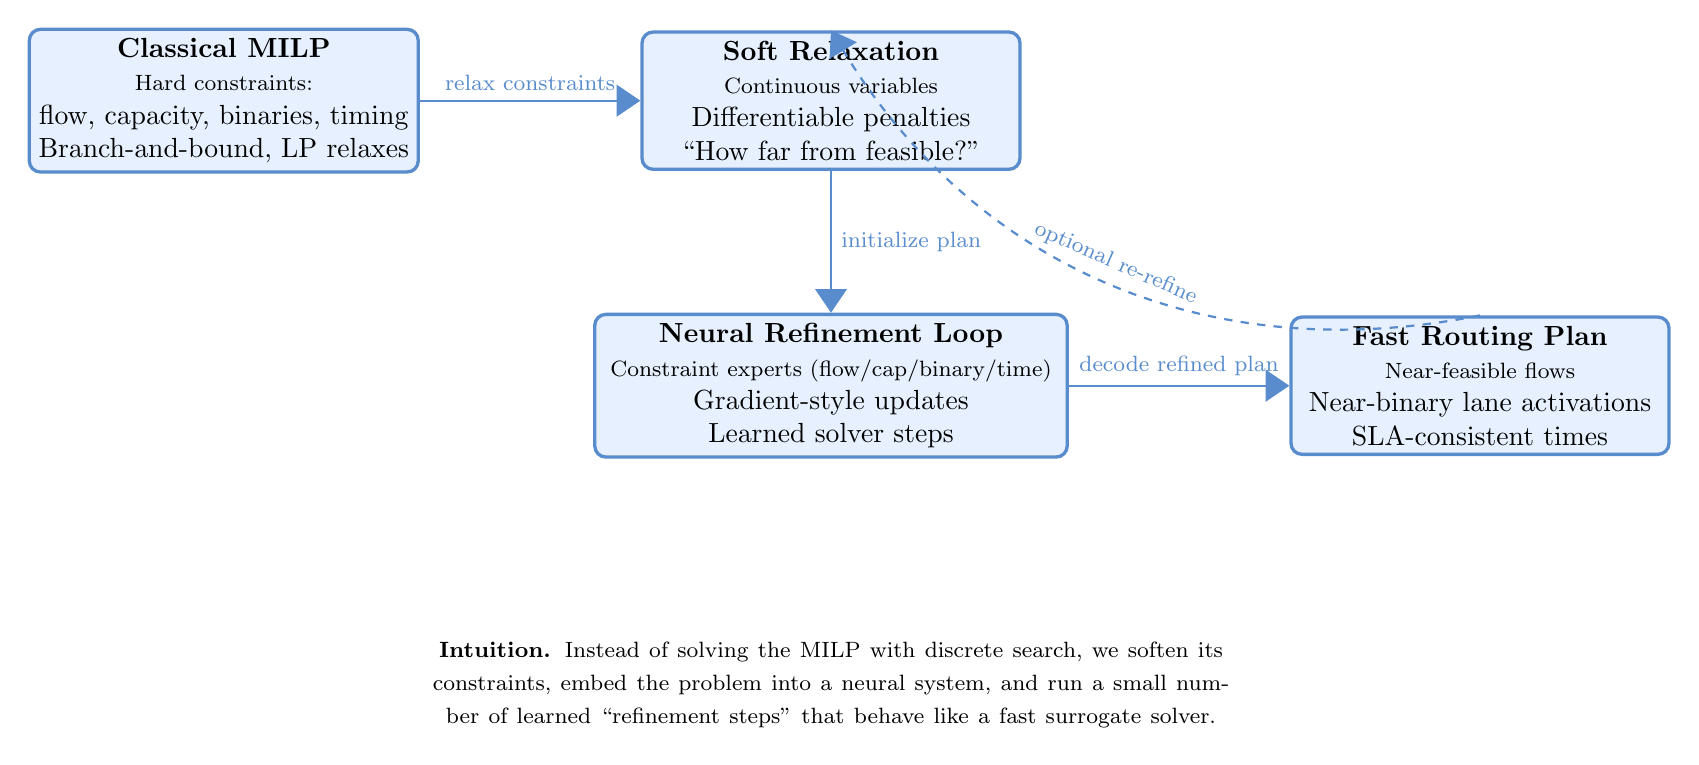
\begin{tikzpicture}[node distance=16mm]

% ---------------------------------------------------------
% Nodes
% ---------------------------------------------------------

% Left: MILP
\node[modulebox] (milp) {%
    \textbf{Classical MILP}\\
    \footnotesize
    Hard constraints:\\
    flow, capacity, binaries, timing\\
    Branch-and-bound, LP relaxes
};

% Middle top: soft relax
\node[modulebox, right=28mm of milp] (soft) {%
    \textbf{Soft Relaxation}\\
    \footnotesize
    Continuous variables\\
    Differentiable penalties\\
    ``How far from feasible?''
};

% Middle bottom: neural refinement loop
\node[modulebox, below=18mm of soft, minimum width=6cm] (refine) {%
    \textbf{Neural Refinement Loop}\\
    \footnotesize
    Constraint experts (flow/cap/binary/time)\\
    Gradient-style updates\\
    Learned solver steps
};

% Right: final plan
\node[modulebox, right=28mm of refine] (out) {%
    \textbf{Fast Routing Plan}\\
    \footnotesize
    Near-feasible flows\\
    Near-binary lane activations\\
    SLA-consistent times
};

% ---------------------------------------------------------
% Arrows
% ---------------------------------------------------------

% MILP -> soft
\draw[arrow] (milp) -- node[above,sloped]{\footnotesize relax constraints} (soft);

% Soft -> refinement
\draw[arrow] (soft.south) -- node[right]{\footnotesize initialize plan} (refine.north);

% Refinement -> output
\draw[arrow] (refine) -- node[above,sloped]{\footnotesize decode refined plan} (out);

% Optional feedback arrow (conceptual)
\draw[arrow, dashed] (out.north) to[bend left=35] node[above,sloped]{\footnotesize optional re-refine} (soft.north);

% Label at bottom
\node[below=22mm of refine, text width=11cm, align=center] (captiontext)
{\footnotesize \textbf{Intuition.} Instead of solving the MILP with discrete search, we soften its constraints, embed the problem into a neural system, and run a small number of learned ``refinement steps'' that behave like a fast surrogate solver.};

\end{tikzpicture}

\caption{From MILP to Neural Surrogate. Hard, combinatorial MILP constraints are replaced by soft, differentiable penalties. A transformer with constraint experts iteratively refines the relaxed solution into a near-feasible routing plan.}
\label{fig:milp_soft_neural}
\end{figure}

%%%%%%%%%%%%%%%%%%%%%%%%%%%%%%%%%%%%%%%%%%%%%%%%%%%%%%%%%%%%
% 4. METHOD
%%%%%%%%%%%%%%%%%%%%%%%%%%%%%%%%%%%%%%%%%%%%%%%%%%%%%%%%%%%%

\section{Method}

\subsection{Architecture Overview}
% Diagram (optional), general flow.

\subsection{Constraint Expert Mixture}
% Show experts specializing:
% - capacity expert
% - flow expert
% - temporal expert
% - feasibility expert

\subsection{Soft Integer Relaxation}
% Sigmoid with temperature
% STE rounding at inference.

\subsection{Latent Gradient Refinement}
% Define energy function
% Gradient update steps.

%%%%%%%%%%%%%%%%%%%%%%%%%%%%%%%%%%%%%%%%%%%%%%%%%%%%%%%%%%%%
% 5. TRAINING
%%%%%%%%%%%%%%%%%%%%%%%%%%%%%%%%%%%%%%%%%%%%%%%%%%%%%%%%%%%%

\section{Training}

% Loss function
% Dataset generation
% Training hyperparameters
% Batch construction

%%%%%%%%%%%%%%%%%%%%%%%%%%%%%%%%%%%%%%%%%%%%%%%%%%%%%%%%%%%%
% 6. EXPERIMENTS
%%%%%%%%%%%%%%%%%%%%%%%%%%%%%%%%%%%%%%%%%%%%%%%%%%%%%%%%%%%%

\section{Experiments}

\subsection{Setup}
% VRP 50/100/200 node

\subsection{Baselines}
% MILP, greedy, neural CO, ablations

\subsection{Results}
% Tables, plots

\subsection{Ablations}
% No experts, no soft relaxation, no refinement

%%%%%%%%%%%%%%%%%%%%%%%%%%%%%%%%%%%%%%%%%%%%%%%%%%%%%%%%%%%%
% 7. ANALYSIS
%%%%%%%%%%%%%%%%%%%%%%%%%%%%%%%%%%%%%%%%%%%%%%%%%%%%%%%%%%%%

\section{Analysis}

% Constraint specialization visualization
% Latent optimization trajectory

%%%%%%%%%%%%%%%%%%%%%%%%%%%%%%%%%%%%%%%%%%%%%%%%%%%%%%%%%%%%
% 8. CONCLUSION
%%%%%%%%%%%%%%%%%%%%%%%%%%%%%%%%%%%%%%%%%%%%%%%%%%%%%%%%%%%%

\section{Conclusion}

% Summary & future work

%%%%%%%%%%%%%%%%%%%%%%%%%%%%%%%%%%%%%%%%%%%%%%%%%%%%%%%%%%%%
% REFERENCES
%%%%%%%%%%%%%%%%%%%%%%%%%%%%%%%%%%%%%%%%%%%%%%%%%%%%%%%%%%%%

\bibliographystyle{plain}
\bibliography{references}

%%%%%%%%%%%%%%%%%%%%%%%%%%%%%%%%%%%%%%%%%%%%%%%%%%%%%%%%%%%%
% APPENDIX
%%%%%%%%%%%%%%%%%%%%%%%%%%%%%%%%%%%%%%%%%%%%%%%%%%%%%%%%%%%%

\appendix

\section{Appendix A: Extended Method}

\section{Appendix B: Additional Experiments}

\end{document}
